\chapter{Design}

\section{Introduction} % (fold)
\label{sec:introduction}

Today the web has become the central point of all applications. With presence of Internet, users can use many applications without needing to install the program on their machine. Technologies such as JavaScript, HTML, CSS are evolving rapidly and has been created an opportunity for the users of world wide web to have a more pleasant experience. Therefore fast and robust application plays an important role in attracting users and convincing them to migrate from installing the programs on their machine and instead use their browsers. In order to build robust web applications,  one must implement new state of the art software engineering designs.

\subsection{Purpose} % (fold)
\label{sub:purpose}

This chapter describes architecture design of `Virtual Assistance' application. It is intended to describe the design of the system fully enough to allow future contributors of the project to clearly understand of how the software is expected to be build. Design chapter will provide overview and description of the system and relations between the components and user interaction. 

\subsection{Scope} % (fold)
\label{sub:scope}
The scope of `AssistU' software design is formulated for base level system which work for a proof of concept, for the use of writing a scientific articles that provides planning, organizing tasks, discussing and suggestions.



\section{Use Cases} % (fold)
\label{sec:system_overview}
\subsection{Actors} % (fold)
\label{sub:actors}
\subsubsection{Student/Researcher User} 
The Student/Researcher is a main user of the application. Without this user, the rest of the actors cannot come in to exist. This user can make use of all the features extensively. For example Student/Researcher can create a project, upload templates and document, invite others, make a planning, discuss a topic with other collaborators, create a to-do-list of what has to be done for the project and get information on how to write a scientific article.

\subsubsection{Reviewer User} 
This actor is able to use all the features as well but most of the attention is given to review student's work. Reviewer come into existence when He/She gets invited by a Student/Researcher into the project. Actions that can be performed by reviewer is to download the document, comment and upload back and discuss a topic on certain  section of the project. He ofcourse can make use of planning and todo feature to create his own events and tasks.

\subsubsection{Guest User} 
Guests are those who are interested to join certain projects. They are meant to do certain actions such as view and download a document and join a discussion to give their comments. Moreover the rest of the features are also open for this actor to make use of if intended.

\subsubsection{Administrative User} 
Administrator of the application represents the operator of the system, extract logs, reply to email requests by client about account and retrieval and security.

\subsection{List of Use Cases} % (fold)
\label{sub:list_of_use_cases}
% TODO: Main use cases of each projects are here
\subsubsection{Student/Researcher User} 
\begin{itemize}
	\item Create/Leave/Archive Project
	\item Invite new members
	\item Search for an Article
	\item Upload/Download/Delete Document
	\item Delete uploaded files
	\item Create project planning
	\item Create to-do list
	\item Create/edit/comment discussion
	\item Make use of suggestions

\end{itemize}
\subsubsection{Reviewer User} 
\begin{itemize}
	 

	\item Join/Leave a project
	\item Download/upload/Delete Document
	\item Create/comment on discussions
\end{itemize}

\subsubsection{Guest User} 
\begin{itemize}
	
	\item Join/Leave a project
	\item Download Document
	\item create/comment on discussions
\end{itemize}	
\subsubsection{Administrative User} 
\begin{itemize}
	\item Add/Remove/Edit user	\item Download logging info
\end{itemize}
\subsection{Use Case Diagrams} % (fold)
\subsubsection{Student/Researcher User} 

\begin{center}
\centering
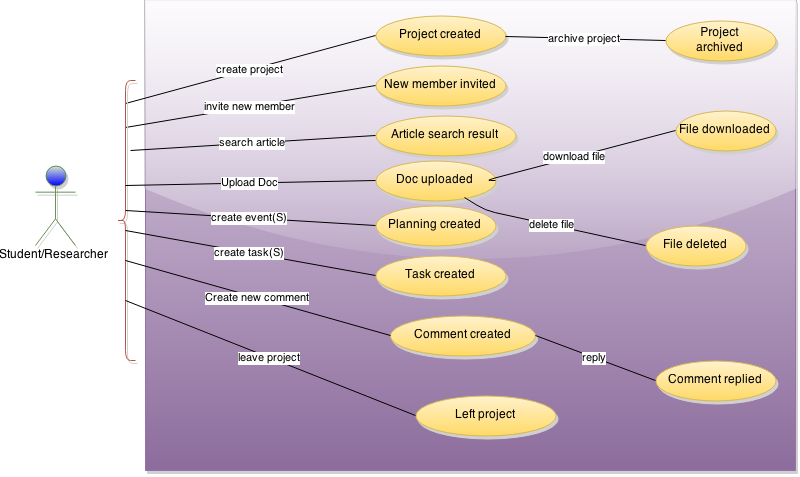
\includegraphics[scale=0.3]{./img/dsgn_img/USECASE1.png}	
\end{center}

% subsection subsection_name (end)

\subsubsection{Reviewer User} 
\begin{center}
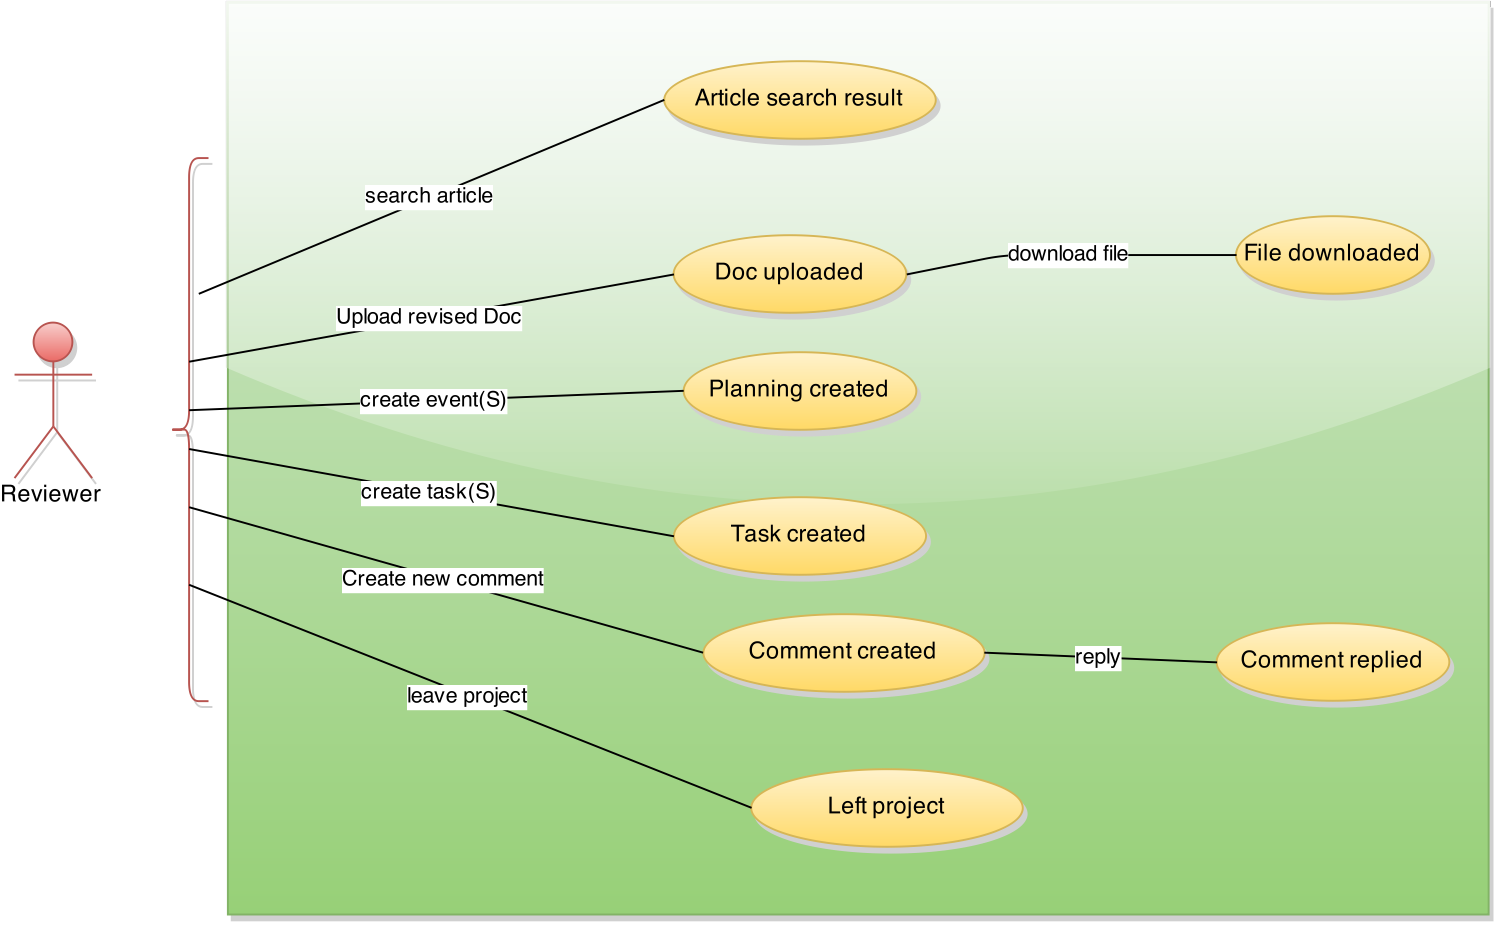
\includegraphics[scale=0.3]{./img/dsgn_img/USECASE2.png}
	
\end{center}

\subsubsection{Guest User} 
\begin{center}
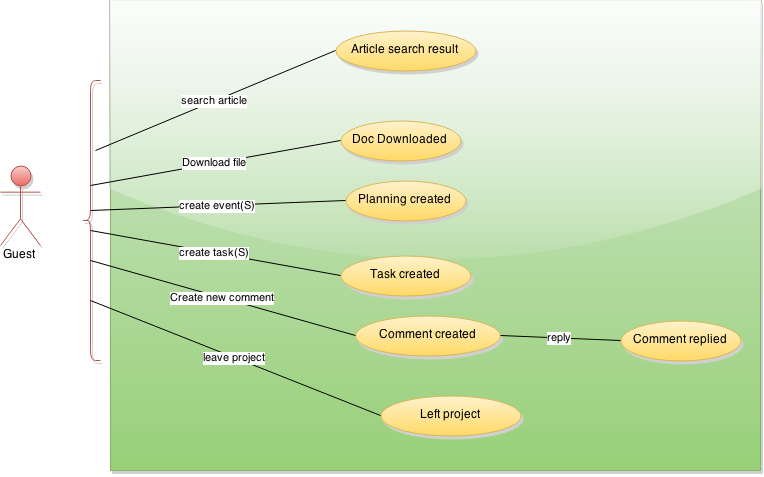
\includegraphics[scale=0.3]{./img/dsgn_img/USECASE4.png}
	
\end{center}

\subsubsection{Administrator User} 
\begin{center}
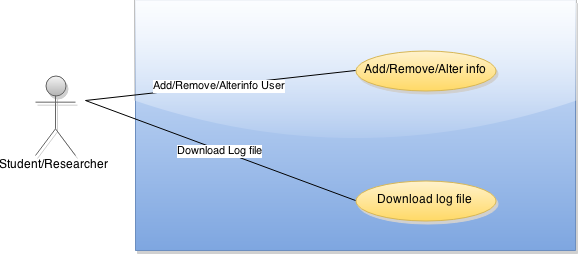
\includegraphics[scale=0.3]{./img/dsgn_img/USECASE3.png}
	
\end{center}
% subsection list_of_use_cases (end)

% subsection actors (end)

\section{System Architecture} % (fold)
\label{sec:system_architecture}
For the purpose of modularity , Model view controller design(MVC) is adopted for the application. In this section, MVC design of the system is shown in the form of diagram and it's sub-component will be discussed. MVC is chosen to be very suitable for web architecture since it promises low coupling and high cohesion between components of the systems and gives room for easier extension or modification of a specific component.
\subsection{Architectural Design} % (fold)
\label{sub:arichtectural_design}
%

In the app folder of this application, there are three packages defined. namely Model, View and Controller. 
\begin{center}
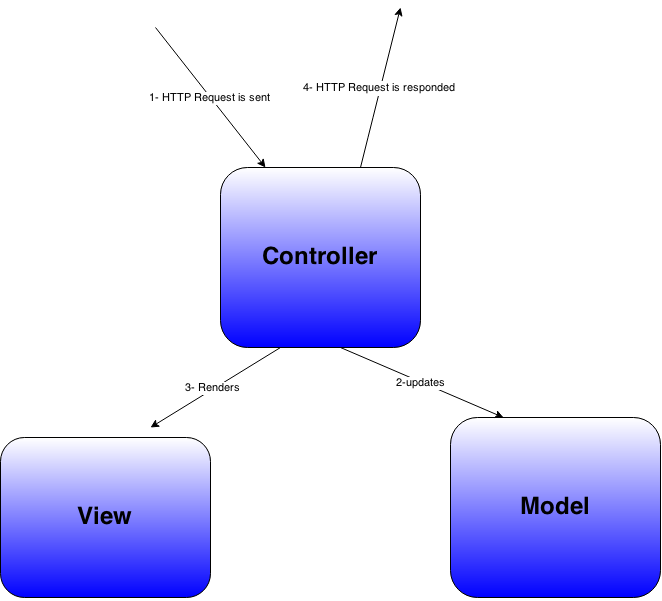
\includegraphics[scale=0.3]{./img/dsgn_img/MVCdiag.png}
	
\end{center}

Image above is showing that the system architecture divides into three separate layers. The model which represents the information, The view that makes these information available for the user and Controller that responds to user actions and processes them. \\
In the next section we will explain more in-dept about each layer and explain what are their sub-components. 

\subsection{Model} % (fold)
\label{sub:design_rationale}
The model is meant to keep track of changes in the states of the application such as when user adds new project or make a new event in the calendar then the related model will notifies it's associated view and controller in the application about the changes. There are also bunch of operational method that lies inside the model package and these operations(static methods) are meant to find information on the database and to update certain information upon user or controller actions.

\subsubsection{Relational Model Diagram}

In order to give a general overview of system model layer, a graphical representation of Entity Relationship(ER) diagram is designed to show the relationship of entities to each other.



\begin{center}
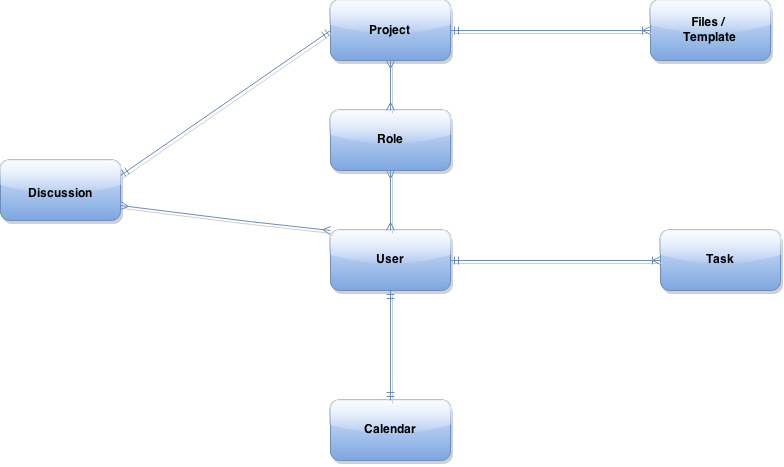
\includegraphics[scale=0.3]{./img/dsgn_img/RMA.png}
	
\end{center}

\subsubsection{Model description}
\paragraph{User}
User model holds all attributes of a user in the application. Users are identified in the program by their email address which is unique. Almost all the models are dependent on user model because non of the model can exist without existence of a user in the application. User attributes consist of unique email, name, password etc.

\paragraph{Project}

Project model is another important model since many other models are related to it. User will need to create a project in order to start his/her project. Informations that are mainly processed in this model are name of the project, project creation date, list of members

\paragraph{Role}

Role model is designed in order to distinguish between users involving in the project. User can only take one role in the project. 

\paragraph{Task} % (fold)
As it appears from its name, Task holds to-do information of a specific user. Single task has name , and due date and a boolean variable to know if user has completed the task.

\paragraph{Calendar} % (fold)

Calendar creates an event for a user. It is meant for the user to have complete planning for the project. An event consist of name, description, start date and end date. 


\paragraph{Discussion} % (fold)
 Members of the project needs to discuss their project , This model will hold such a information. It has a subject and description with time stamp to keep track of time-line of the discussions. 


\paragraph{Document Files} % (fold)

Document files holds information on the version and name of the specific file that is uploaded in the project. any file that is uploaded will have a unique version and this is how files with the same name are identified among project.


\subsection{View} % (fold)
View is the gate for the user to interact with the application. Design of the View layer is simple and minimalistic. Image snapshot of view's sub-components are shown next.
\subsubsection{Login}

\begin{center}
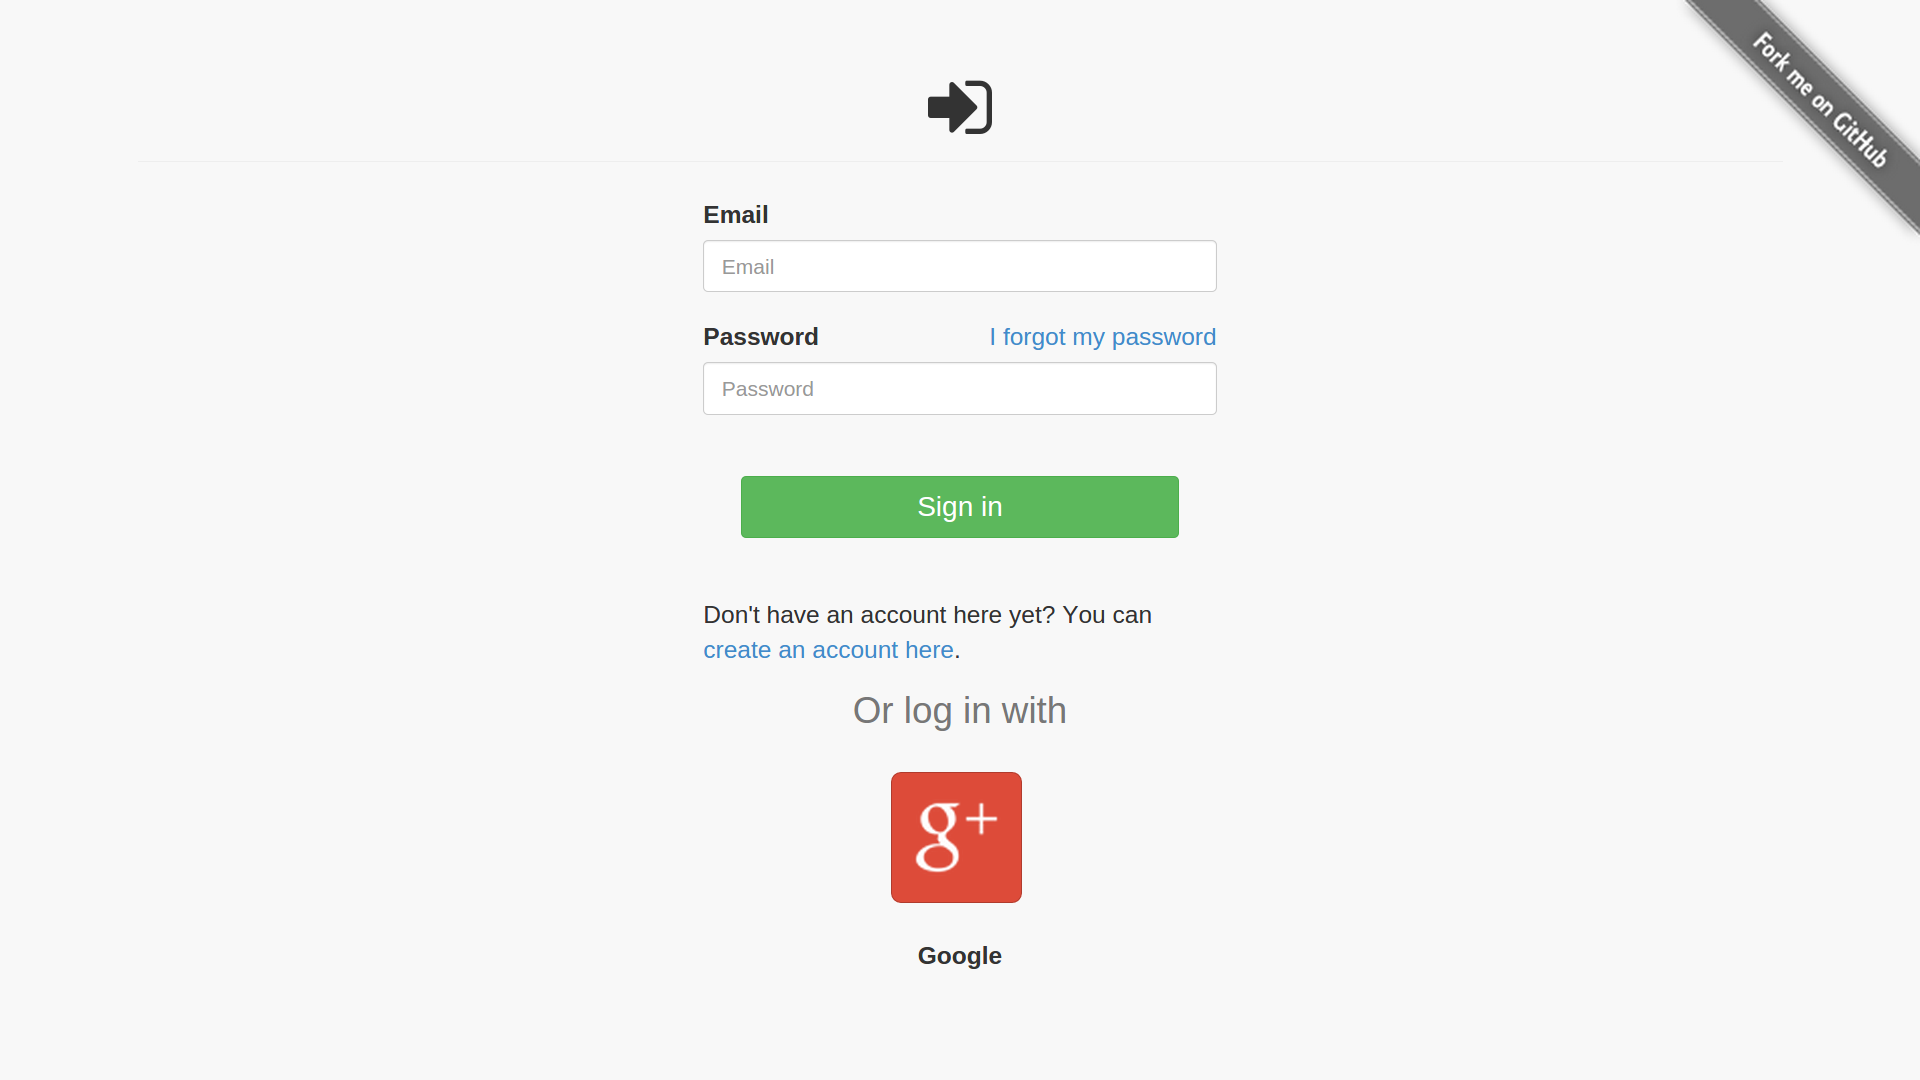
\includegraphics[height=200px, width=350px]{./img/dsgn_img/login.png}
	
\end{center}

\subsubsection{Dashboard}

\begin{center}
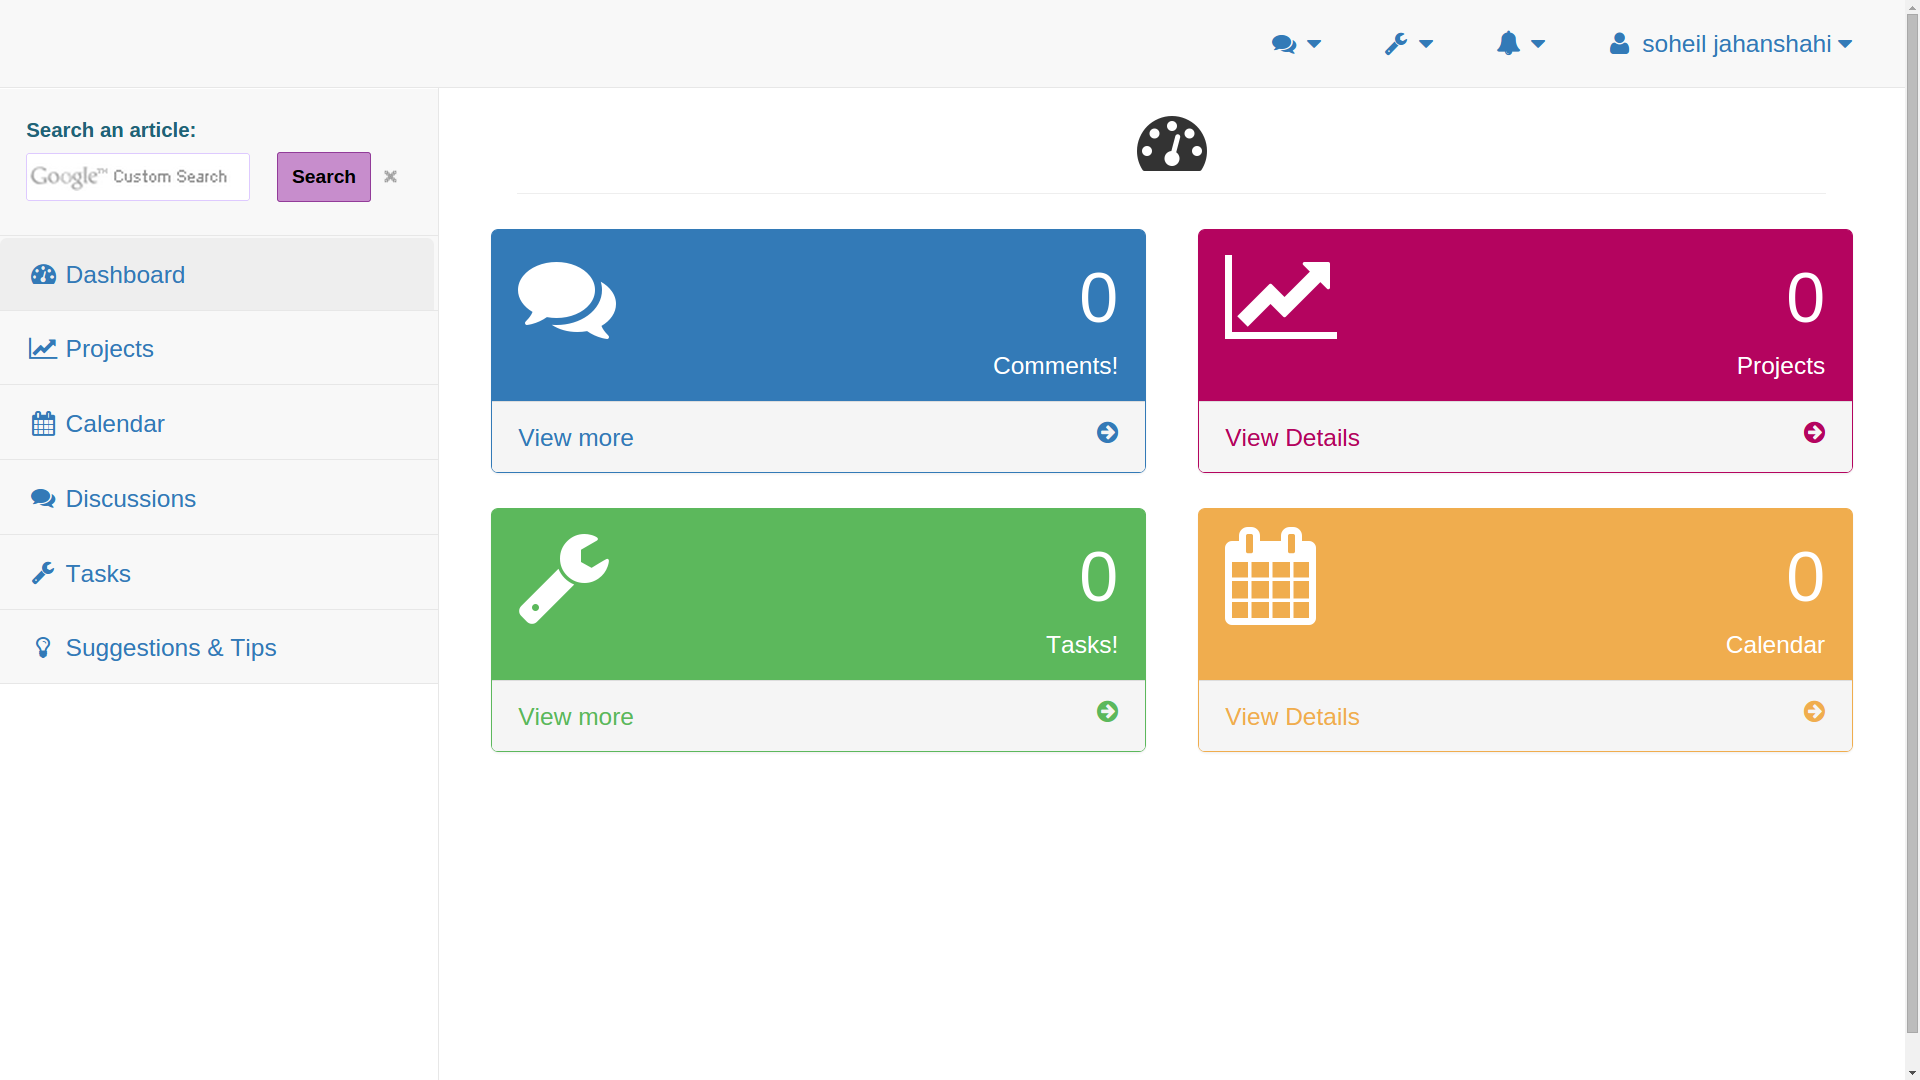
\includegraphics[height=200px, width=350px]{./img/dsgn_img/dashboard.png}
	
\end{center}

\subsubsection{Project}

\begin{center}
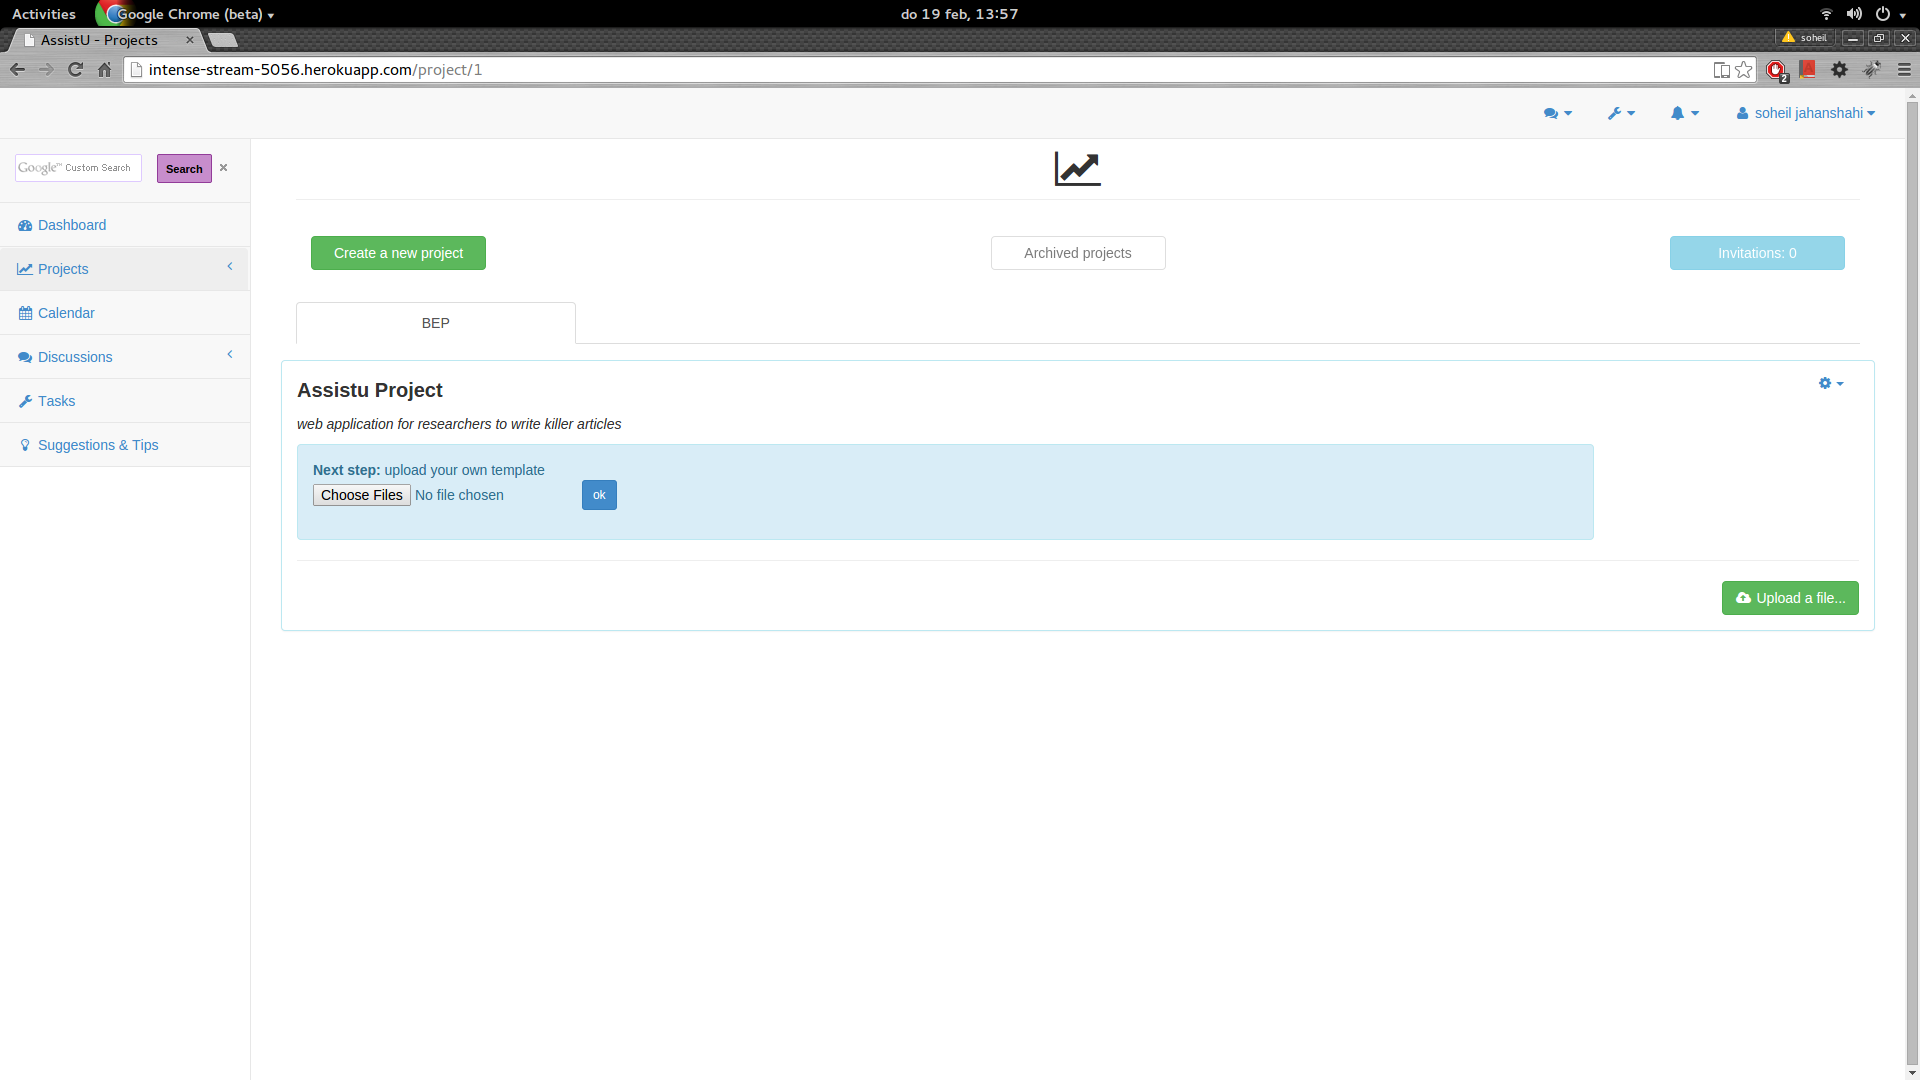
\includegraphics[height=200px, width=350px]{./img/dsgn_img/project.png}
	
\end{center}
\subsubsection{Discussion}

\begin{center}
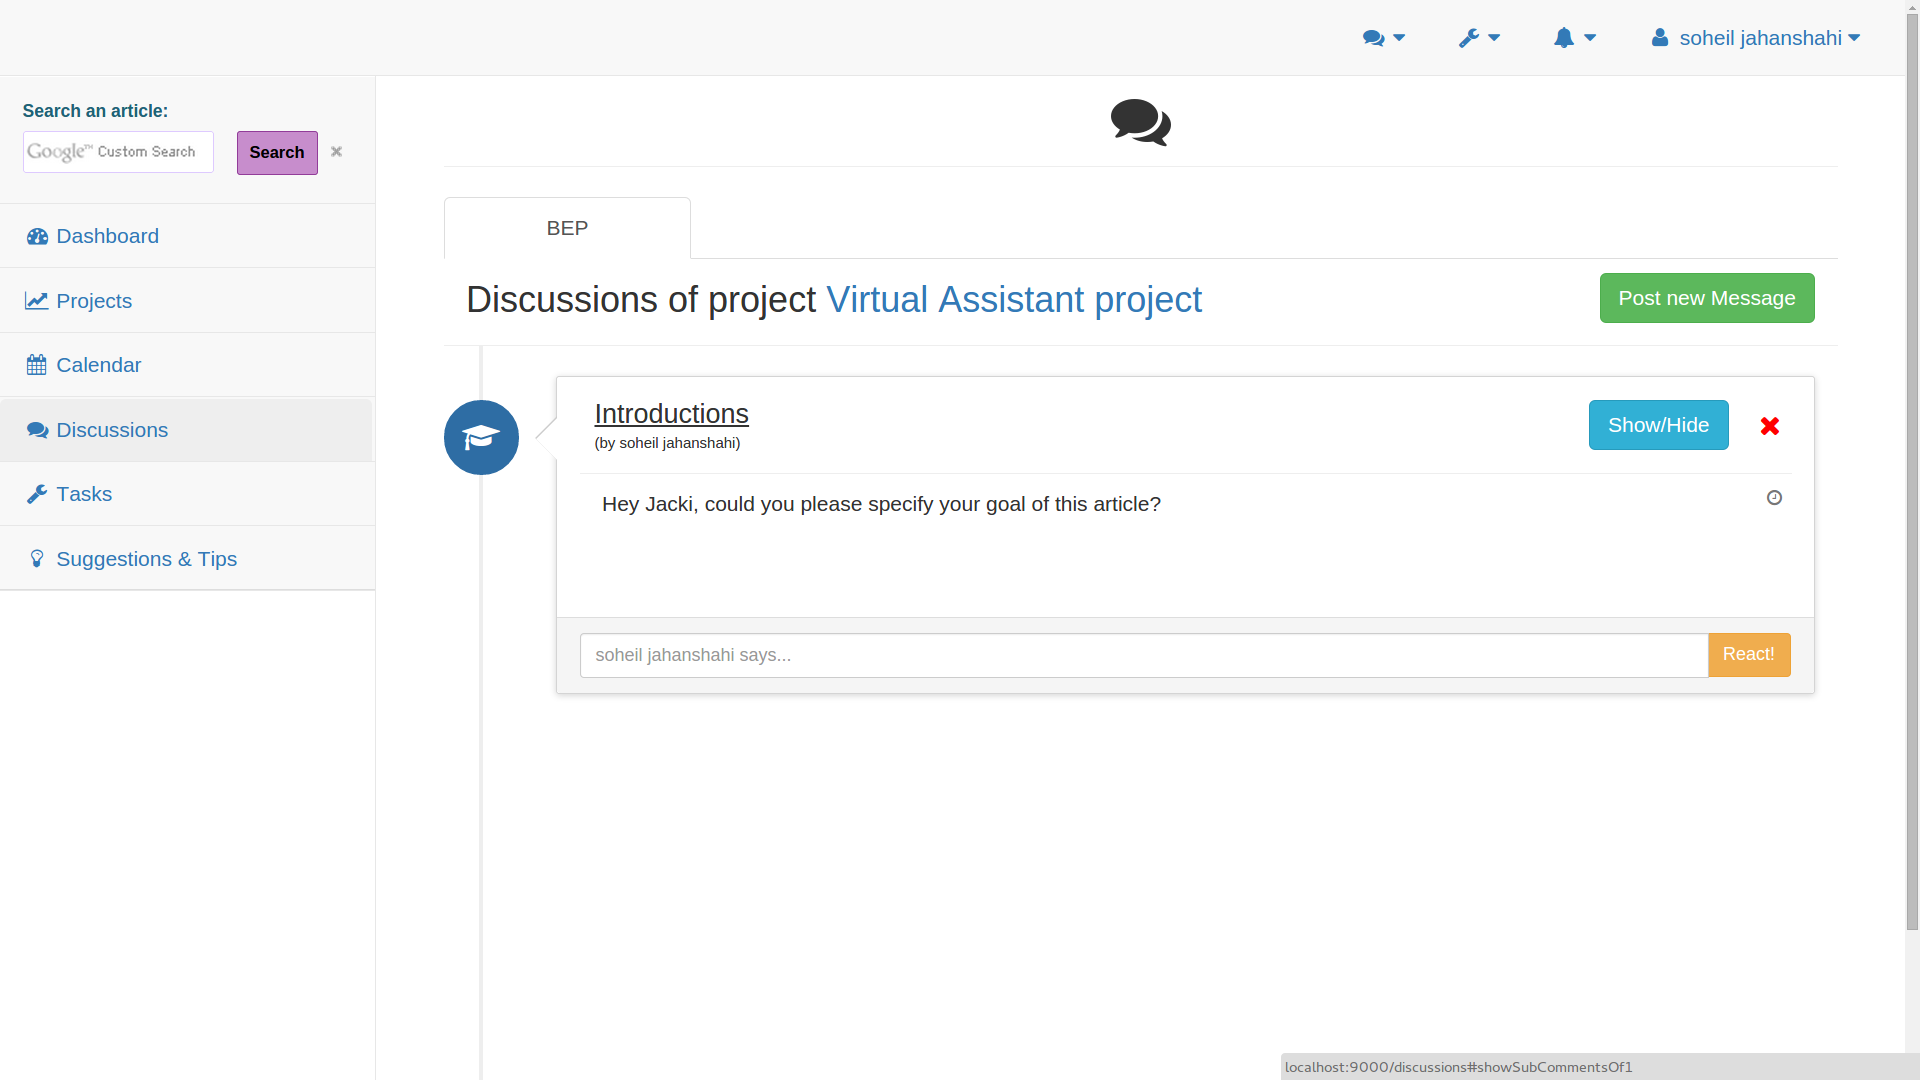
\includegraphics[height=200px, width=350px]{./img/dsgn_img/discussion.png}
	
\end{center}

\subsubsection{Calendar}

\begin{center}
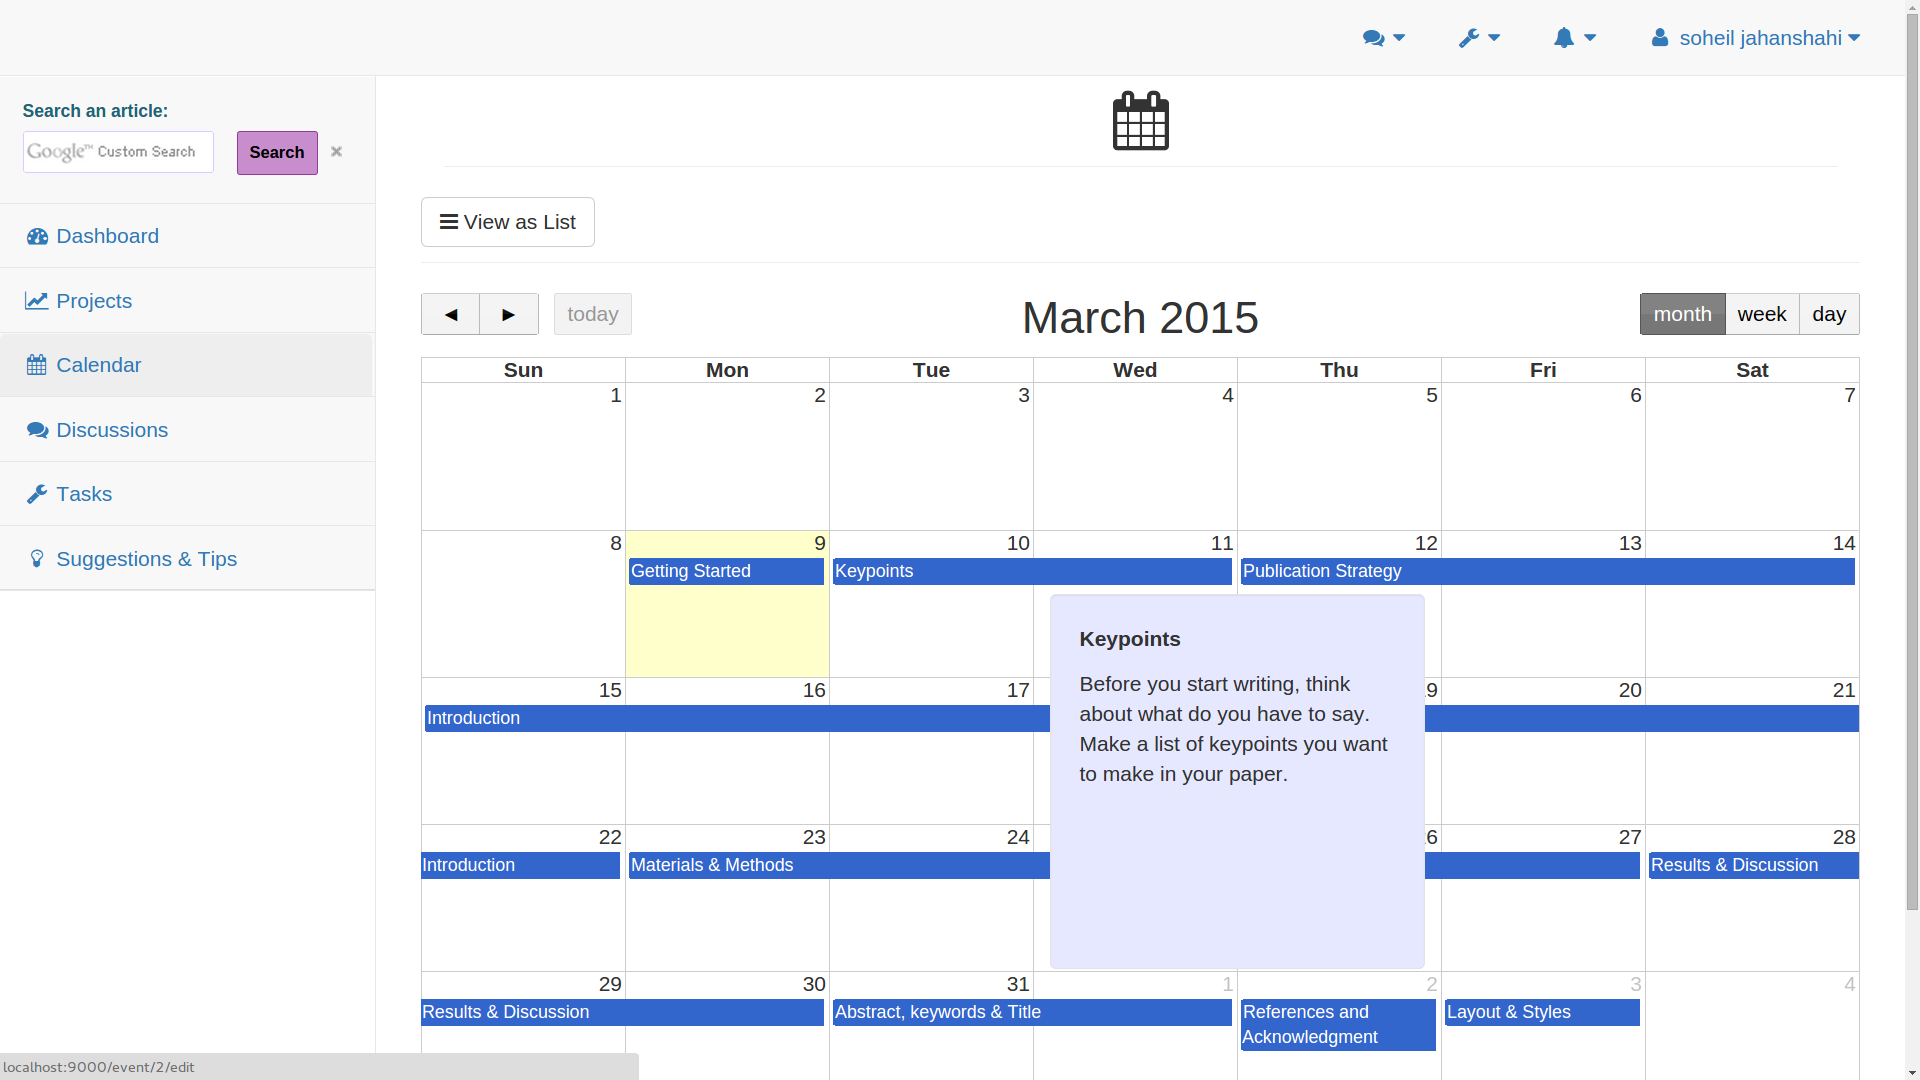
\includegraphics[height=200px, width=350px]{./img/dsgn_img/calendar.png}
	
\end{center}

\subsubsection{Task}

\begin{center}
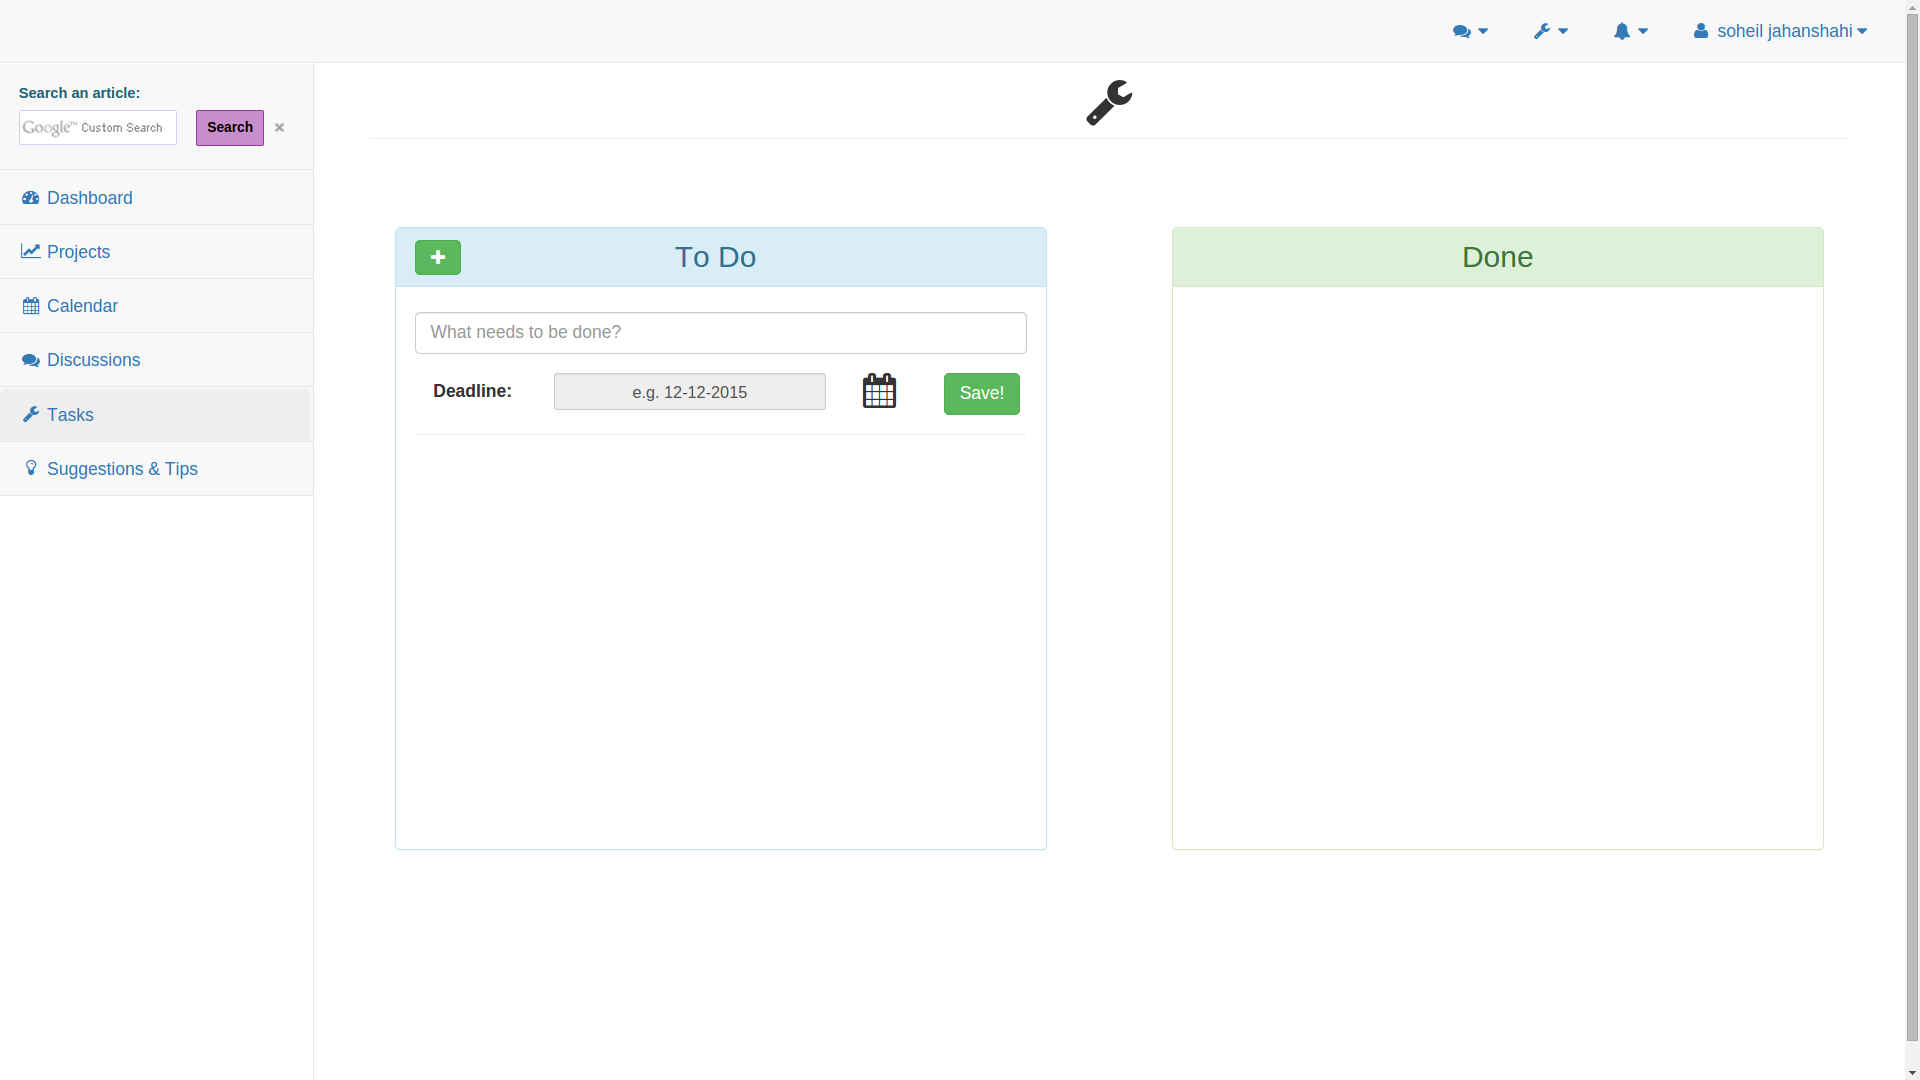
\includegraphics[height=200px, width=350px]{./img/dsgn_img/task.png}
	
\end{center}

\subsubsection{Suggestions}

\begin{center}
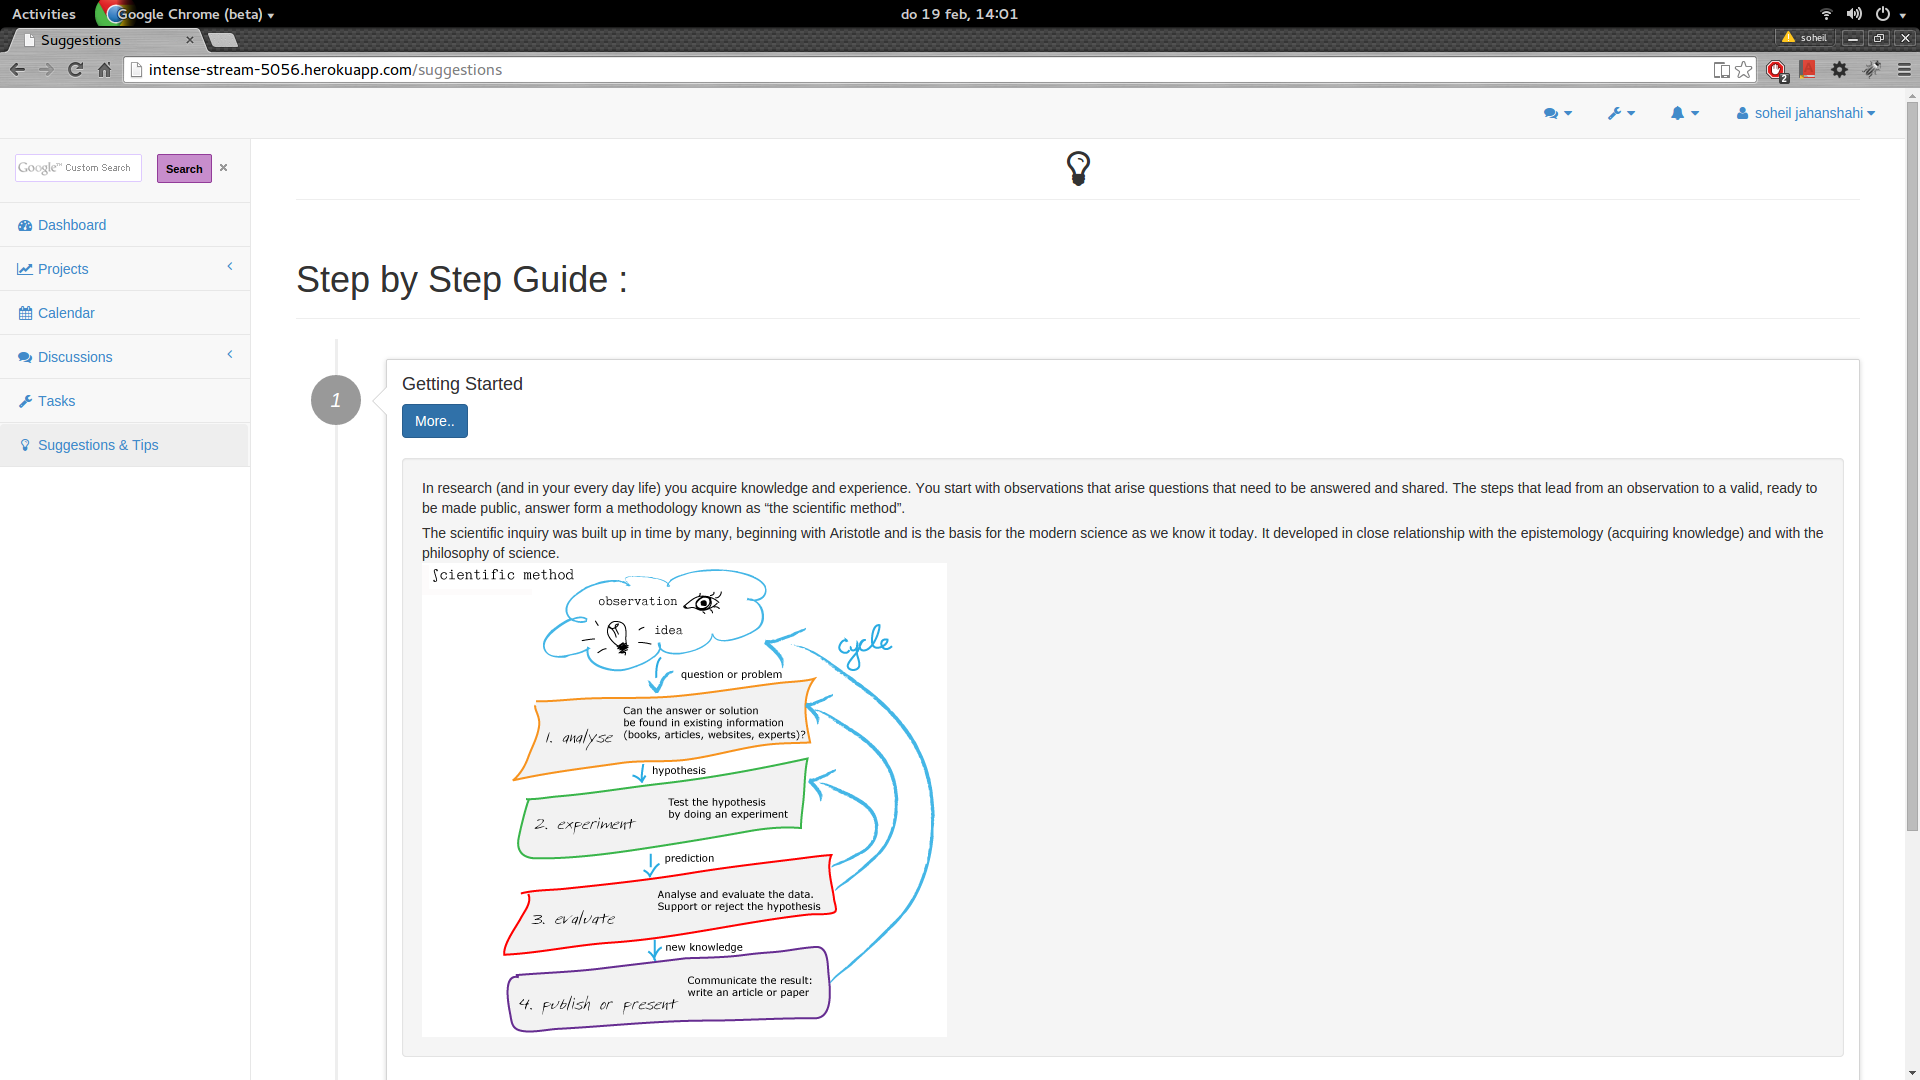
\includegraphics[height=200px, width=350px]{./img/dsgn_img/suggestions.png}
	
\end{center}





\subsection{Controller}

Controllers are the brain of the application, It will handle the request that is requested by the user from view and responds to it accordingly. At time controller might need to update the model if there is any change in the state of the information.